\newcommand{\pluginName}{Historical Simulator}
\newcommand{\pluginVersion}{1.0.0}

\input{../../../DocumentationTemplate/TemplateL3}

\begin{document}
\PluginTitle{\pluginName}{\pluginVersion}

\section{Introduction}
\emph{Historical Simulator} plug-in allows you to simulate underlying asset trajectories by using historical time series (i.e. stored in CSV files on the file system).
Possible applications can be to check the behaviour of a deal using historical realizations, or to build cases where Monte Carlo simulation is mixed with deterministic trajectories.

\section{How to use the plug-in}
In the Fairmat user interface when adding a new stochastic process
you will find the additional option \emph{Historical Simulator}.
The process input parameters (See also Figure~\ref{fig.HistoricalSimulatorGUI}) are the following:
\begin{itemize}
\item \textbf{File path:} the source file where the historical series are memorized
\item \textbf{Start date:} the date $D$, within the input file which will be used as reference for the forward simulation starting at Simulation Start Date $S$.  In practice, the simulator translates forward the stock prices of $S-D$ days.
\end{itemize}

\begin{figure}[ht]
\begin{center}
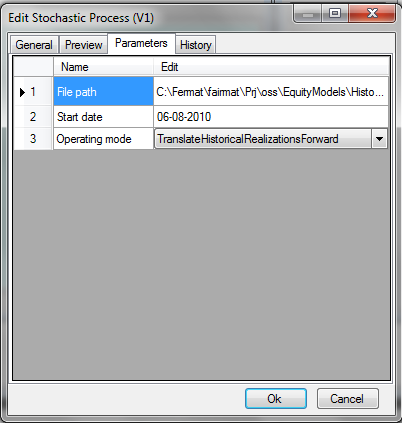
\includegraphics[width=0.48\textwidth]{./figures/HistoricalSimulatorEdit.png}
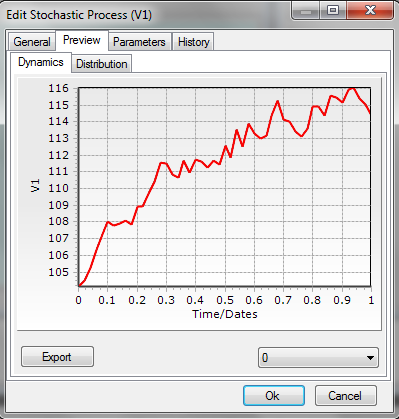
\includegraphics[width=0.48\textwidth]{./figures/HistoricalSimulatorPreview.png}
\caption{Historical Simulator GUI: input parameters editor and preview.}
\label{fig.HistoricalSimulatorGUI}
\end{center}
\end{figure}

\subsection{File Format details}
In the actual version of the plug-in, time series must be defined on  CSV files (using spaces, tabs or semicolon as separators). 
\begin{small}
\begin{verbatim}
01/01/2010	100.1	1203.2	43.4
02/01/2010	102.3	1213.0	43.7
03/01/2010	101.2	1209.1	43.8
...
\end{verbatim}
\end{small}





\end{document}
